\section{Tape-Out}
\label{sec:tapout}

We intended to finish the chip design portion of this project in the previous thesis, however slip in the timeline caused us to miss the first tape-out deadline and submission date for that thesis. A large part of the slippage was caused by having to redesign the buck-boost converter regulator loop to implement peak current-mode control due to issues with the previously implemented average current-mode control. Even with the extended timeline it was difficult to complete the design before the deadline leading us rush some aspects of the design and remove nonessential features like the over-temperature protection circuit we designed.

\subsection{Buck-Boost Converter}
The layout of the buck-boost converter can be seen in  \autoref{fig:BBlayout} with annotations showing the rough floorplan of the circuit. Surrounding the converter are the four large switching transistors which increased significantly in size between initial planning in the previous thesis and to what we ultimately implemented. The exact values and sizes are listed in \autoref{tab:spec_pmos} and \autoref{tab:spec_nmos}. The largest contributor to the losses in the power-stage surprisingly are the metal resistances which increased the the theoretical $R_{DS,on}$ of the \ac{PMOS} transistors from \qty{58.3}{\milli\ohm} to an effective \qty{240}{\milli\ohm} considering trace resistances. These metal resistances could not be further minimized through wider traces as the limiting factor was the maximum copper density for manufacturing. \\
The large empty space above the error amplifier in \autoref{fig:BBlayout} was initially intended for a temperature sensing circuit in order to measure the rough temperature of power electronics and to disable operation in case of an over temperature event. Due to the tight timeline we opted to not layout this circuit as we were already significantly behind schedule and needed the time to finish the layout of other critical circuits. 

\begin{table}[H]
    \centering
    \begin{tabular}{|c|c|c|}
        Characteristic & Planned Value & Implemented Value \\
        \hline
		 Typ. $R_{DS,on}$ & \qty{113}{\milli\ohm}  & \qty{58.3}{\milli\ohm} \\
         \# of Transistors & \qty{4834}{}  & \qty{9408}{} \\
		 Width & \qty{96.7}{\milli\meter} & \qty{188.2}{\milli\meter}\\
		 Size & \qty{1000.2}{\micro\meter} x \qty{486.8}{\micro\meter} & \qty{1228.8}{\micro\meter} x \qty{764.4}{\micro\meter}
    \end{tabular}
    \caption{Specifications of the power \ac{PMOS}}
    \label{tab:spec_pmos}
\end{table}

\begin{table}[H]
    \centering
    \begin{tabular}{|c|c|c|}
        Characteristic & Planned Value & Implemented Value \\
        \hline
		 Typ. $R_{DS,on}$ & \qty{72.8}{\milli\ohm} & \qty{37}{\milli\ohm} \\
         \# of Transistors & \qty{2800}{}  & \qty{6080}{} \\
		 Width & \qty{56}{\milli\meter} & \qty{121.6}{\milli\meter} \\
		 Size & \qty{641.4}{\micro\meter} x \qty{483.1}{\micro\meter} & \qty{972.8}{\micro\meter} x \qty{688}{\micro\meter}
    \end{tabular}
    \caption{Specifications of the power \ac{NMOS}}
    \label{tab:spec_nmos}
\end{table}

\begin{figure}[h]
    \centering
    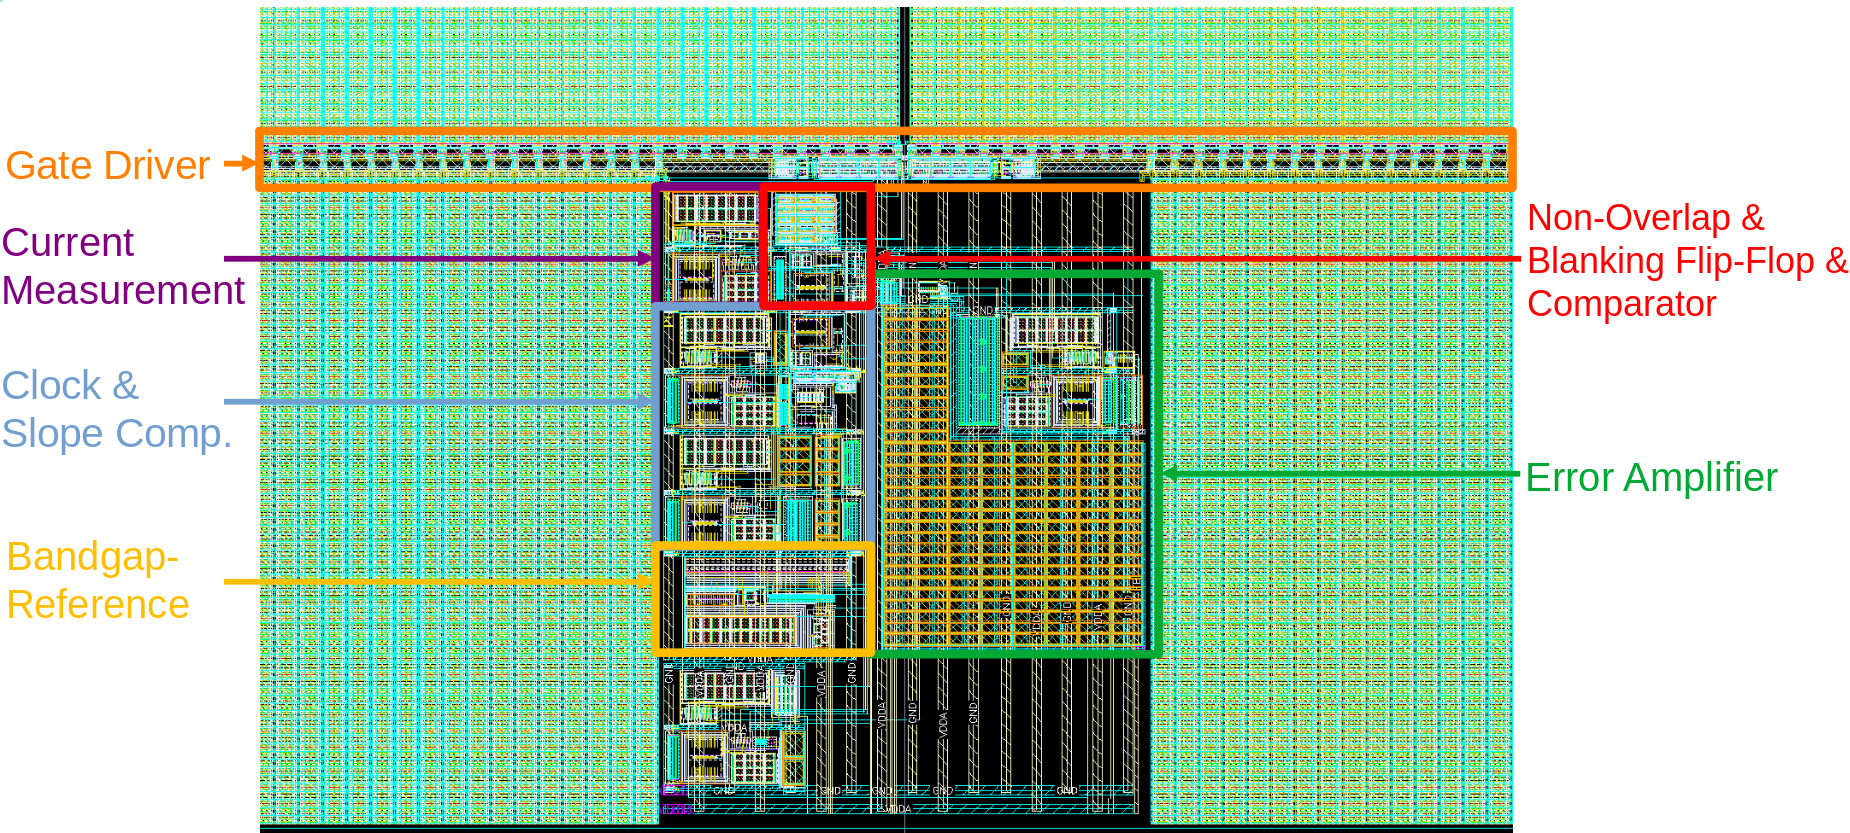
\includegraphics[width=1\textwidth]{../ASIC-DESIGN-2/images/07_DCDC/BuckBoostLayout.png}
    \caption{Layout of the buck-boost converter regulator surrounded by the large power stage transistors}
    \label{fig:BBlayout}
\end{figure}

\clearpage

\subsection{Overall Chip Floorplan}
As can be seen in \autoref{fig:chiplayout}, this design is significantly pad limited as opposed to core limited. The entire lower right corner is unused and in general the lower third is sparsely populated opposed the the upper two thirds which is entirely filled the the buck-boost converter. The large switching transistors were maximized to reduce conversions losses and take up the majority of the chips area. A large number of pads are used in parallel to meet our current handling capabilities and not exceed the recommendation of \qty{50}{\milli\ampere} per pad. In the bottom left the digital circuitry for the \ac{SPI} periphery and internal registers can be seen as well as supporting circuitry like the \ac{POR} and bandgap voltage reference. 
\begin{table}[H]
    \centering
    \begin{tabular}{|c|c|}
        Property & Value \\
        \hline
        Function & Buck-Boost Converter \\
        Package & QFN48 7x\qty{7}{\milli\meter} \\
        Process & X-Fab \qty{350}{\nano\meter} \\
		Size & \qty{2712}{\micro\meter} x \qty{2952}{\micro\meter} \\
        Area & \qty{8.006}{\milli\meter\squared}
    \end{tabular}
    \caption{ASIC Properties}
    \label{tab:spec_asic}
\end{table}
\begin{figure}[h]
    \centering
    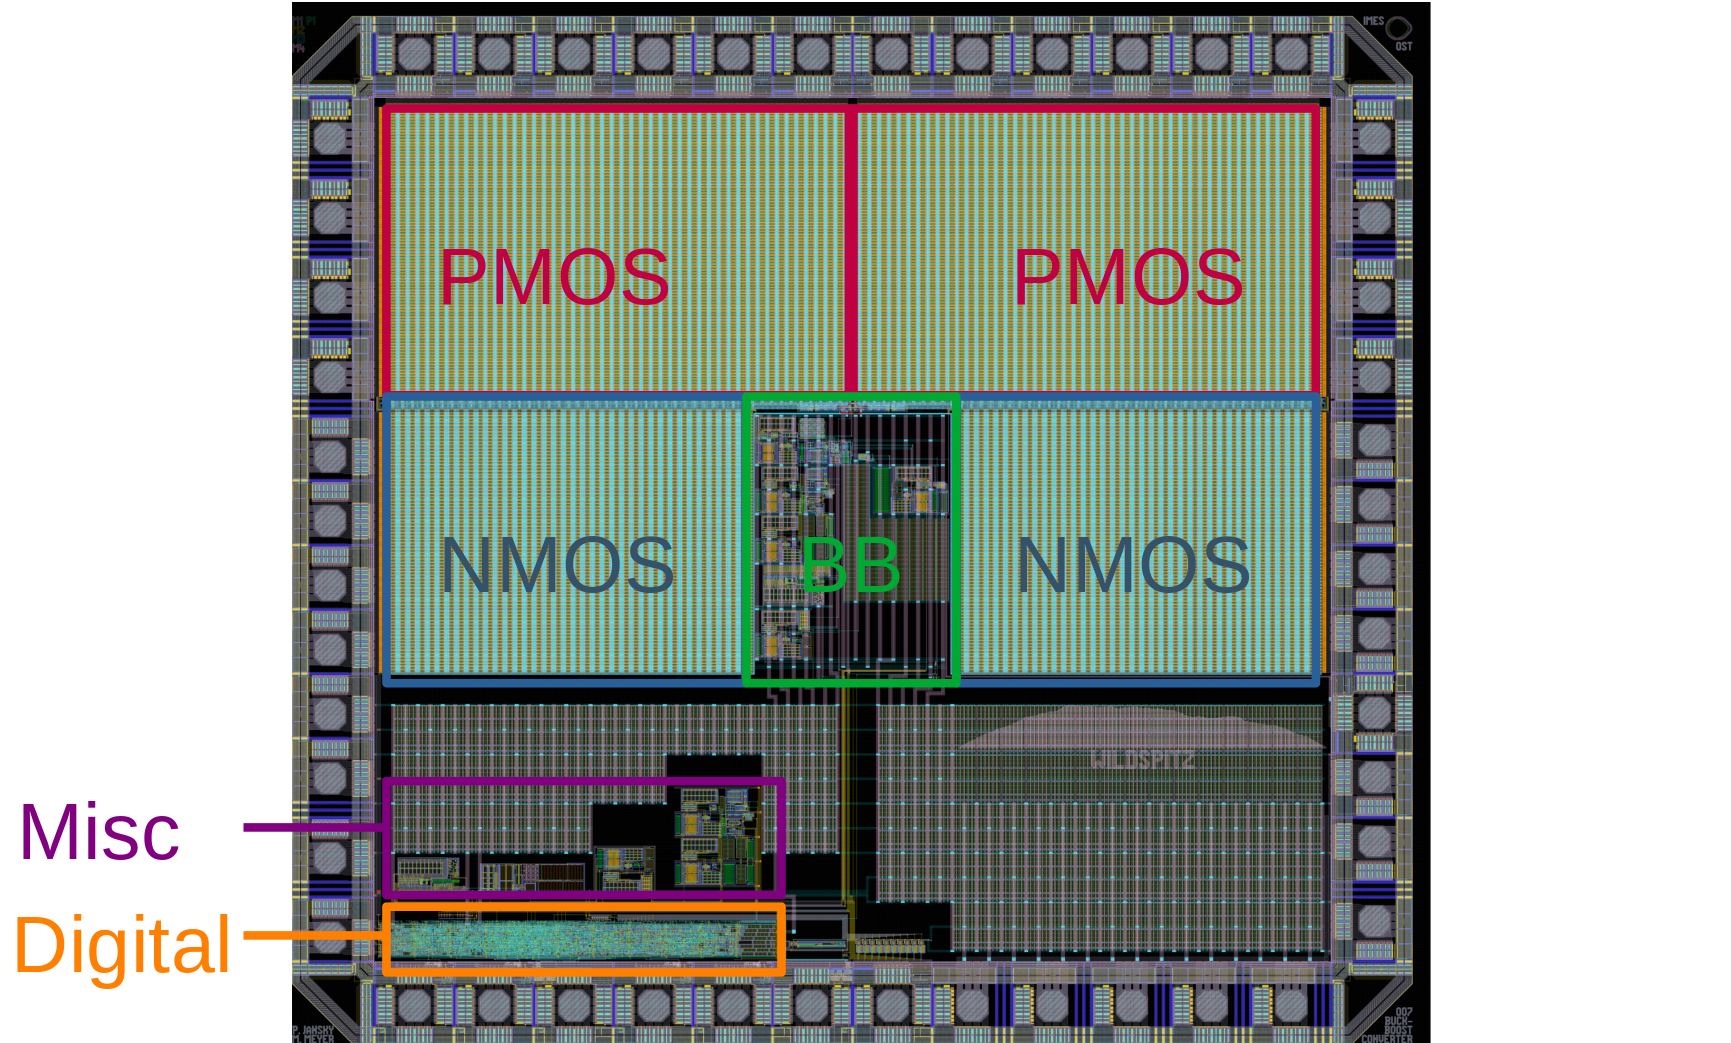
\includegraphics[width=1\textwidth]{../ASIC-DESIGN-2/images/07_DCDC/ChipLayout.png}
    \caption{Floorplan of the entire chip with annotations}
    \label{fig:chiplayout}
\end{figure}

